\quad Na poniższym wykresie jest przedstawiona tabela ilości 
zaklasyfikowanych do prostej punktów w zależności od precyzji zminnej (float32, float64) i 
$\varepsilon$.
zbiorze testowym specjalnie dla tego celu (zbiór punktów na prostej).
$ 10^4$ losowych punktów w przestrzeni $\mathbb{R}^2$ dla $ x \in \langle -1000,1000 \rangle$ leżących na prostej wyznaczonej przez wektor $ \overrightarrow{ab}$.   
    Gdzie $ a = (-1.0, 0.0)$, $ b = (1.0, 0.1)$.
\\
\begin{figure}[hbt]
    \centering
    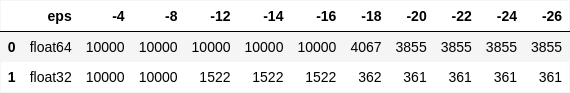
\includegraphics[scale=0.6]{eps.png}
    \caption*{Tabela 6: Porównanie precyzji float64 i float 32.}
\end{figure}
\par
\quad Patrząc na porównanie precyzji float64 z float32, możemy dojść do wniosku, 
że float64 daje (jak wypadało się spodziewać) dużo większą precyzje obliczeń. 
Widoczna jest poważna różnica w obliczeniach już dla $\varepsilon = 10^{-12}$. 
Dlatego na potrzeby algorytmów geometrycznych zalecane jest 
używanie float64.